\section{Results}
\label{sec:results}

\subsection{The committed history of case C14}
\label{sec:res-committed}

The bank of case C14 breaches the standardised outlier test at all three valuation dates: the ratio of the loss of economic value under the worst shock to Tier~1 capital is \cOneFourRatioA{} at 2021-Q4, \cOneFourRatioB{} at 2022-Q2 and \cOneFourRatioC{} at 2022-Q4, against the limit of 0.15 (Table~\ref{tab:c14-history}). The breach flag is therefore one at every date and does not vary, which is the first thing to know about what the test can show on this case. The fitted weighted average maturity of the wholesale deposits is \cOneFourWamA{}, \cOneFourWamB{} and \cOneFourWamC{} years at the three dates. The engine, run on this series with the flags of the outlier test, returns not evaluated at 2021-Q4, where the history has one date, red at 2022-Q2 with one flagged change, and red at 2022-Q4 with two, the changes at 30 June and 31 December 2022; these are the committed rows of the product, reproduced to the last digit by running the function on the committed series and on the fitted series rebuilt from the raw inputs, which differ from the committed ones by \cOneFourRebuiltMaxDiff{} years. The requested core share and the requested core maturity of the same deposits, which the case states and holds at 0.6 and 5 years, are green, and so is the fitted series when its breach flags are set to false. Prediction H1 holds.

\begin{table}[htbp]
\centering
\footnotesize
\caption{The committed history of case C14, the wholesale deposits of the bank at three valuation dates: the standardised outlier ratio and its breach flag, the fitted weighted average maturity (WAM), the proposed test on the history up to each date, and the two other behavioural tests of the engine rerun on the committed inputs.}
\label{tab:c14-history}
\resizebox{\textwidth}{!}{%
\begin{tabular}{lrlrlll}
\toprule
Date & EVE risk measure / Tier 1 & Breach & Fitted WAM (years) & Proposed test (flagged changes) & Weight stability & EVE with and without \\
\midrule
2021-12-31 & 0.341 & yes & 4.759 & not evaluated & red & red \\
2022-06-30 & 0.209 & yes & 4.205 & red (1) & amber & red \\
2022-12-31 & 0.181 & yes & 5.000 & red (2) & red & red \\
\bottomrule
\end{tabular}}
\end{table}


\begin{figure}[htbp]
\centering
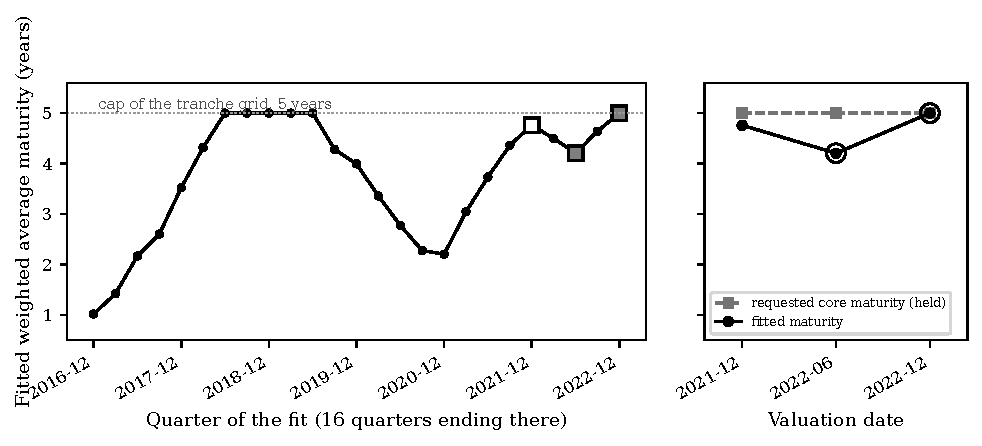
\includegraphics[width=0.92\textwidth]{history}
\caption{The weighted average maturity of the wholesale deposits fitted at each quarter from 2016-Q4 to 2022-Q4 on the last 16 quarters of the bank's deposit cost and of the Treasury tranche yields (left), with the three committed valuation dates marked and the two dates flagged by the proposed test ringed, and the series at those three dates beside the requested core maturity that the case holds fixed (right).}
\label{fig:history}
\end{figure}

Figure~\ref{fig:history} places the three dates in the full fitted series. The series has \realFits{} fits; its median absolute change between consecutive fits is \realMedianChange{} years and its largest is \realMaxChange{} years; \realZeroShare{} of the changes are zero, which happens where the solution sits at the 5-year cap of the tranche grid, and the weighted average maturity is at the cap at \realCapShare{} of the dates. The figure shows what Proposition~\ref{prop:degeneracy} states: a fitted series moves at nearly every date, so the red rows reflect the re-estimation and the breach, and not a decision. The two other behavioural tests of the engine, run on the committed inputs, read the same history differently. The stability test of the weights is red at 2021-Q4, with a largest sup-norm distance of \cOneFourStabStatA{} and a change of up to \cOneFourStabYearsA{} years in the weighted average maturity, amber at 2022-Q2 (\cOneFourStabStatB{}) and red at 2022-Q4 (\cOneFourStabStatC{}), so it flags the date at which the proposed test has nothing to say. The comparison of the economic value with and without the behavioural treatment is red at the three dates, with differences of \cOneFourWwStatA{} and \cOneFourWwStatC{} of Tier~1 at the first and the last, and none of them is a hidden breach, since the behavioural measure breaches the outlier test as well as the contractual one. None of the three tests reads the timing of an assumption against the timing of a breach except the proposed one, and on this case none can say whether the bank altered its assumptions, because the behaviour is synthetic.

\subsection{Constructed and enumerated histories}
\label{sec:res-constructed}

The engine agrees with the definition on all \constructedN{} constructed histories of Table~\ref{tab:constructed}, of which \constructedAgree{} gave the expected light: green for the parameter held through a breach, for the change with no breach, for the change before the breach and for a breach at the earlier date only; red for the change at the breach and for two changes at two breaches; not evaluated for a single date. Prediction H2 asks for more than examples, and the enumeration provides it: on every one of the \gridTotal{} histories of a binary grid of \gridLengths{} dates, each pattern of changes crossed with each pattern of flags (\gridSix{} histories of six dates), and on \randomN{} random histories with ties at a cap, the number of disagreements between the engine and Equation~\eqref{eq:count} is \gridBad{}. The light was red exactly when the count was positive in all of them.

\begin{table}[htbp]
\centering
\footnotesize
\caption{Constructed histories with a known answer, the parameter values and breach flags at three valuation dates, the light expected from the definition of the test and the light returned by the engine; the single-date history has one value and one flag.}
\label{tab:constructed}
\resizebox{\textwidth}{!}{%
\begin{tabular}{lllllr}
\toprule
History & Parameter & Breach flags & Expected & Engine & Flagged changes \\
\midrule
parameter held through a breach & $(4, 4, 4)$ & $(1, 1, 1)$ & green & green & 0 \\
change with no breach & $(4, 4.5, 5)$ & $(0, 0, 0)$ & green & green & 0 \\
change before the breach & $(4, 4.5, 4.5)$ & $(0, 0, 1)$ & green & green & 0 \\
change at the breach & $(4, 4, 4.5)$ & $(0, 0, 1)$ & red & red & 1 \\
breach at the earlier date only & $(4, 4.5, 4.5)$ & $(1, 0, 0)$ & green & green & 0 \\
two changes at two breaches & $(4, 4.5, 5)$ & $(0, 1, 1)$ & red & red & 2 \\
change at the first date (no previous date) & $(4, 4, 4)$ & $(1, 0, 0)$ & green & green & 0 \\
a single date & $(4)$ & $(1)$ & not evaluated & not evaluated & -- \\
\bottomrule
\end{tabular}}
\end{table}


Table~\ref{tab:last-digit} shows the convention the test inherits from its definition. A parameter held at 4 years with Gaussian noise of standard deviation $10^{-16}$ added at each date is still green, because the noise is smaller than the spacing of floating-point numbers at 4 and the sum rounds back; noise of \noiseFirstRed{} or more turns the light red at the two breach dates, and the held value recomputed as the sum of 0.1 and 0.2 differs from 0.3 in the last digit and is red too. A parameter that is recomputed at each date through a different order of operations, even if its mathematical value is constant, is flagged, so an implementation of the test on a stated parameter must hold it as the number that was decided and not as the result of a calculation.

\begin{table}[htbp]
\centering
\footnotesize
\caption{The effect of the last digit of a held parameter on the proposed test: a parameter held at 4 years through a 12-quarter history with two breach dates, to which Gaussian noise of the stated size is added at each date; the last row is the same value recomputed as 0.1 plus 0.2 and as 0.3, two floating-point numbers that differ.}
\label{tab:last-digit}
\begin{tabular}{lll}
\toprule
Noise on the held value (standard deviation) & Engine & Flagged changes \\
\midrule
0 & green & 0 \\
1e-16 & green & 0 \\
1e-13 & red & 2 \\
1e-09 & red & 2 \\
1e-06 & red & 2 \\
$0.1+0.2$ against $0.3$ & red & 2 \\
\bottomrule
\end{tabular}
\end{table}


\subsection{A stated parameter with planted changes}
\label{sec:res-stated}

Table~\ref{tab:main-results} gives the comparison in the base cell, with unrelated changes at 0.10 per quarter and a breach prevalence of 0.25, on \statedN{} histories per arm with a mean of \statedMeanM{} breach dates. The proposed test flags \statedAltEngine{} of the histories with a planted change at a breach date (lower end of the interval \statedAltLoEngine{}\,\%), as Proposition~\ref{prop:separation} requires, and \statedNullEngine{} (\statedNullLoEngine{} to \statedNullHiEngine{}\,\%) of the histories whose changes are unrelated to the breaches. The breach-agnostic count flags the same share of the alternative histories and \statedNullAny{} of the null ones, so the conjunction with the breach flag removes about half of the false flags at no cost in detection. The Fisher test flags \statedNullFisher{} of the null histories and \statedAltFisher{} of the alternative ones, the Mann--Whitney test \statedNullMw{} and \statedAltMw{}, and the Welch test \statedNullWelch{} and \statedAltWelch{}: they hold a size far below the nominal 5\,\% and detect a fraction of the planted changes. In the area under the ROC curve the ordering is not the same: the Fisher test (\statedAucFisher{}) and the Mann--Whitney test (\statedAucMw{}) rank the histories slightly better than the count of the proposed test (\statedAucEngine{}), which has only the values of its count to rank with, and the Welch test is lower (\statedAucWelch{}).

\begin{table*}[htbp]
\centering
\footnotesize
\caption{The proposed test and the comparators run on the same histories: on a stated parameter (4,000 histories per arm, changes unrelated to the breach at 0.10 per quarter, breach prevalence 0.25) and on a re-estimated parameter (2,000 banks, breach prevalence 0.25, a 2-year lengthening planted at breach dates); false-flag and detection rates with 95\% Wilson intervals, and the area under the ROC curve; the tolerance is calibrated at 5\% on 1,000 separate banks.}
\label{tab:main-results}
\resizebox{\textwidth}{!}{%
\begin{tabular}{lcccccc}
\toprule
\multicolumn{1}{l}{} & \multicolumn{3}{c}{Stated parameter} & \multicolumn{3}{c}{Re-estimated parameter} \\
\cmidrule(lr){2-4}\cmidrule(lr){5-7}
Detector & False flags (\%) & Detection (\%) & AUC & False flags (\%) & Detection of +2 years (\%) & AUC \\
\midrule
Proposed test & 34.8 (33.4, 36.3) & 100.0 (99.9, 100.0) & 0.908 & 82.2 (80.5, 83.9) & 100.0 (99.8, 100.0) & 0.579 \\
Any change & 68.8 (67.3, 70.2) & 100.0 (99.9, 100.0) & 0.863 & 92.5 (91.3, 93.6) & 100.0 (99.8, 100.0) & 0.536 \\
Fisher exact test & 0.1 (0.1, 0.3) & 13.2 (12.2, 14.3) & 0.922 & 2.1 (1.5, 2.8) & 4.1 (3.3, 5.1) & 0.596 \\
Mann--Whitney test & 2.6 (2.1, 3.1) & 48.0 (46.5, 49.6) & 0.914 & 7.2 (6.2, 8.5) & 31.4 (29.5, 33.5) & 0.796 \\
Welch test & 0.3 (0.2, 0.6) & 26.8 (25.5, 28.2) & 0.761 & 6.0 (5.1, 7.2) & 28.9 (27.0, 30.9) & 0.696 \\
Calibrated tolerance & -- & -- & -- & 3.9 (3.1, 4.8) & 18.0 (16.4, 19.7) & 0.937 \\
Calibrated tolerance, look-ahead & -- & -- & -- & 4.5 (3.6, 5.4) & 17.2 (15.6, 18.9) & 0.925 \\
Weight stability (engine) & -- & -- & -- & 49.8 (47.6, 52.0) & -- & -- \\
\bottomrule
\end{tabular}}
\end{table*}


The false-flag rate of the proposed test over the \statedCells{} cells of Table~\ref{tab:stated-grid} runs from \statedNullMin{} to \statedNullMax{}, at the lowest rate of unrelated changes with the lowest prevalence and at the highest with the highest, so prediction H5, a rate of at most 5\,\%, is refuted in every cell. Equation~\eqref{eq:false-flag}, evaluated with the number of breach dates of the very histories of each cell, lies inside the interval of the measured rate in \bernInside{} of the \bernCells{} cells (prediction H4); the cell outside, $\lambda=0.05$ at prevalence 0.5, has a closed form of \bernOutPred{} and a measured rate of \bernOutObs{}, a difference of \proofGap{} percentage points that is the largest of the grid, and under \bernExtraInside{} of three further seeds of 10,000 histories the closed form is inside the interval. The Fisher and Mann--Whitney tests never exceed \fisherNullMax{} and \mwNullMax{} false flags in any cell. The detection of the Fisher test depends on how many breach dates carry a planted change: with $\pi_m$ at 0.25, 0.5 and 1 it flags \piSweepAFisher{}, \piSweepBFisher{} and \piSweepCFisher{}, the Mann--Whitney test \piSweepAMw{}, \piSweepBMw{} and \piSweepCMw{}, and the Welch test \piSweepAWelch{}, \piSweepBWelch{} and \piSweepCWelch{}, whereas the proposed test flags every history in every cell (\statedAltMinLo{} at the lowest lower bound; prediction H3 holds).

\begin{table*}[htbp]
\centering
\footnotesize
\caption{The stated parameter over the grid of the rate of changes unrelated to the breach ($\lambda$ per quarter), the breach prevalence and the probability of a planted change at a breach date ($\pi_m$), 4,000 histories per arm in each row: the mean number $m$ of breach dates, the false-flag rate of the proposed test predicted by Proposition~\ref{prop:false-flag} and measured, and the detection rates of three detectors.}
\label{tab:stated-grid}
\resizebox{\textwidth}{!}{%
\begin{tabular}{rrrrrcrrr}
\toprule
\multicolumn{4}{l}{} & \multicolumn{2}{c}{Proposed test, false flags (\%)} & \multicolumn{3}{c}{Detection (\%)} \\
\cmidrule(lr){5-6}\cmidrule(lr){7-9}
$\lambda$ & Prevalence & $\pi_m$ & Mean $m$ & Closed form & Measured & Proposed & Fisher & Mann--Whitney \\
\midrule
0.05 & 0.10 & 0.50 & 3.87 & 17.2 & 17.0 (15.8, 18.1) & 100.0 & 13.5 & 57.4 \\
0.05 & 0.25 & 0.50 & 4.42 & 19.4 & 18.7 (17.5, 20.0) & 100.0 & 14.0 & 52.1 \\
0.05 & 0.50 & 0.50 & 5.80 & 25.0 & 27.4 (26.0, 28.8) & 100.0 & 16.3 & 39.5 \\
0.10 & 0.10 & 0.50 & 4.01 & 31.7 & 31.9 (30.4, 33.3) & 100.0 & 11.3 & 51.1 \\
0.10 & 0.25 & 0.50 & 4.37 & 34.3 & 34.8 (33.4, 36.3) & 100.0 & 13.2 & 48.0 \\
0.10 & 0.50 & 0.50 & 5.85 & 43.6 & 42.9 (41.4, 44.5) & 100.0 & 12.6 & 35.1 \\
0.20 & 0.10 & 0.50 & 3.92 & 51.3 & 52.0 (50.5, 53.5) & 100.0 & 8.8 & 43.9 \\
0.20 & 0.25 & 0.50 & 4.38 & 55.4 & 55.2 (53.7, 56.8) & 100.0 & 9.8 & 40.5 \\
0.20 & 0.50 & 0.50 & 5.73 & 66.5 & 66.3 (64.9, 67.8) & 100.0 & 10.2 & 31.8 \\
0.10 & 0.25 & 0.25 & 4.36 & 34.2 & 33.0 (31.6, 34.5) & 100.0 & 2.8 & 31.0 \\
0.10 & 0.25 & 1.00 & 4.48 & 34.8 & 34.1 (32.6, 35.6) & 100.0 & 60.2 & 89.1 \\
\bottomrule
\end{tabular}}
\end{table*}


\begin{figure}[htbp]
\centering
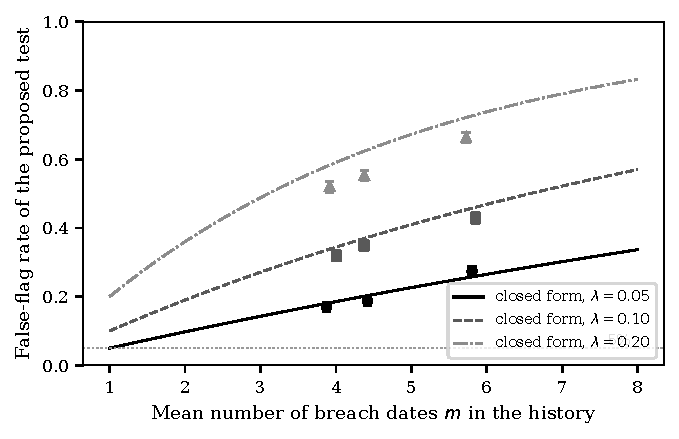
\includegraphics[width=0.62\textwidth]{false-flag}
\caption{The false-flag rate of the proposed test on a stated parameter against the mean number of breach dates in the history, for three rates of unrelated changes, with the closed form of Proposition~\ref{prop:false-flag} as lines and the nine cells of the simulation as markers with their 95\% Wilson intervals; the dotted line is a rate of 5\%.}
\label{fig:false-flag}
\end{figure}

Figure~\ref{fig:false-flag} shows the agreement of the closed form with the nine cells of the grid and the rise of the rate with the number of breach dates; the rate does not depend on the planted changes, which are absent from the null arm. Figure~\ref{fig:operating-points} plots the detection against the false-flag rate of the five detectors over the same cells. The proposed test and the breach-agnostic count sit on the line of full detection with false-flag rates between \statedNullMin{} and \statedNullAnyMax{}, and the three tests sit near the line of no false flags with detection between \opTestsMin{} and \opTestsMax{}; no detector reaches the corner of full detection at a low false-flag rate, because in a history of a dozen quarters a coincidence and a decision cannot be told apart by the dates alone. The figure does not show the tolerance rule, which is not defined on a stated parameter, where every change is a decision and the size of a change is a matter of governance and not of estimation.

\begin{figure}[htbp]
\centering
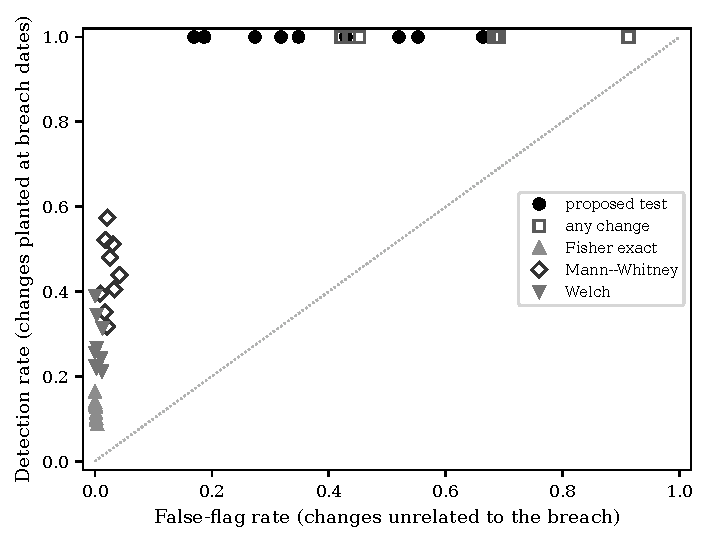
\includegraphics[width=0.66\textwidth]{operating-points}
\caption{Detection rate against false-flag rate of five detectors on a stated parameter, one marker for each of the nine cells of the grid of the rate of unrelated changes and the breach prevalence, with the proposed test at full detection and the three published tests near the line of no false flags.}
\label{fig:operating-points}
\end{figure}

\subsection{A re-estimated parameter}
\label{sec:res-fitted}

The simulated banks are block bootstraps of the real rows, and Table~\ref{tab:realism} compares their changes with those of the real fitted series. Their zero-change share (\simZero{}) and their share of dates at the cap (\simCap{}) are close to the real ones, and their largest change, \simMax{} years on average, is larger than the real \realMaxChange{} years; their median change, \simMedian{} years, is smaller than the real \realMedianChange{} years, which is above the 95th percentile of the simulated medians (\simMedianQNineFive{} years). The simulated changes are thus more often tiny and more often large than the real ones, which are steady, and Figure~\ref{fig:changes-ecdf} shows the distributions. The weight of this difference falls on the calibrated tolerance and is reported where it appears.

\begin{table}[htbp]
\centering
\footnotesize
\caption{The real fitted series of the bank (25 rolling fits from 2016-Q4 to 2022-Q4, and the last 12) against the simulated banks on the properties of the changes that the detectors read; the simulated banks are circular block bootstraps of the 40 real quarterly rows with blocks of 6 quarters.}
\label{tab:realism}
\resizebox{\textwidth}{!}{%
\begin{tabular}{lrrr}
\toprule
Property of the fitted weighted average maturity & Real, 25 fits & Real, last 12 fits & Simulated, mean of 2,000 banks \\
\midrule
Median absolute change (years) & 0.435 & 0.437 & 0.140 \\
Largest absolute change (years) & 0.919 & 0.843 & 1.116 \\
Share of dates with no change & 0.167 & 0.000 & 0.276 \\
Share of dates at the 5-year cap & 0.240 & 0.083 & 0.289 \\
Standard deviation of the level (years) & 1.198 & 0.943 & 0.714 \\
\bottomrule
\end{tabular}}
\end{table}


\begin{figure}[htbp]
\centering
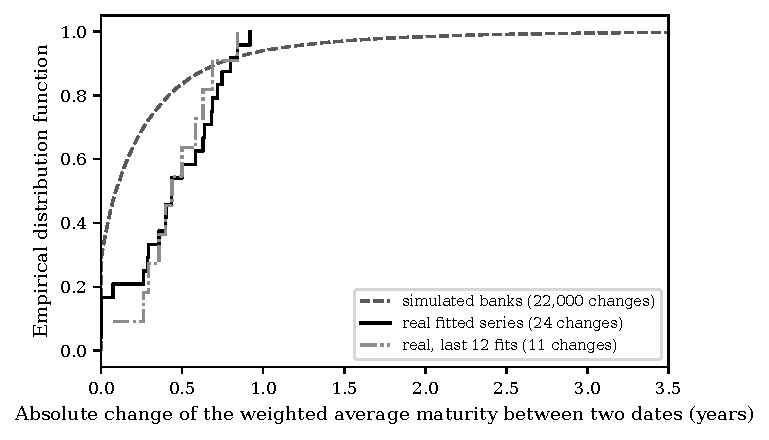
\includegraphics[width=0.62\textwidth]{changes-ecdf}
\caption{The empirical distribution of the absolute change of the fitted weighted average maturity between consecutive dates, for the 22,000 changes of the simulated test banks, the 24 changes of the real fitted series and the 11 changes of its last 12 fits.}
\label{fig:changes-ecdf}
\end{figure}

On the null banks, with a mean of \fitMeanM{} breach dates, the proposed test flags \fitNullEngine{} (\fitNullLoEngine{} to \fitNullHiEngine{}\,\%), and the \fitNullZero{} that it does not flag are those in which all the breach dates are ties, since \tieBanks{} of the banks have at least one tie at a breach date, \tieMean{} on average, because the weighted average maturity repeats at the cap. With a 2-year lengthening planted at breach dates it flags \fitAddCEngine{}, and the area under its ROC curve is \fitAucCEngine{} (\fitAucLoCEngine{} to \fitAucHiCEngine{}), the same at every size of the lengthening from 0.5 to 4 years, which is what Proposition~\ref{prop:degeneracy} predicts: the count is the number of breach dates minus the ties, and a planted change adds a change only where the fitted series was tied. Prediction H6, an area of at least 0.70, is refuted. The breach-agnostic count flags \fitNullAny{} of the null banks and has an area of \fitAucCAny{}. The stability test of the engine is red in \fitNullStab{} of the null banks, so a red result from it is no better evidence of an override. The published tests do better on ranking and worse on size: Table~\ref{tab:fitted-power} shows that the Mann--Whitney test flags \fitNullMw{} of the null banks, above its nominal 5\,\%, and \fitAddCMw{} of the banks with a 2-year lengthening, with an area of \fitAucCMw{}; the Welch test flags \fitNullWelch{} and \fitAddCWelch{}; the Fisher test flags \fitNullFisher{} and \fitAddCFisher{}.

\begin{table*}[htbp]
\centering
\footnotesize
\caption{Detection of a persistent lengthening of the fitted weighted average maturity planted at breach dates (breach prevalence 0.25): flag rate in percent and area under the ROC curve (separated by a slash) for each size of the lengthening, on 2,000 simulated banks and on 2,000 draws of breaches and overrides on the real fitted series of the bank; the tolerance is calibrated on the simulated banks.}
\label{tab:fitted-power}
\resizebox{\textwidth}{!}{%
\begin{tabular}{llrrrrr}
\toprule
Detector & Banks & False flags (\%) & +0.5 year & +1 year & +2 years & +4 years \\
\midrule
Proposed test & simulated & 82.2 & 100.0 / 0.58 & 100.0 / 0.58 & 100.0 / 0.58 & 100.0 / 0.58 \\
Proposed test & real series & 100.0 & 100.0 / 0.50 & 100.0 / 0.50 & 100.0 / 0.50 & 100.0 / 0.50 \\
Any change & simulated & 92.5 & 100.0 / 0.54 & 100.0 / 0.54 & 100.0 / 0.54 & 100.0 / 0.54 \\
Any change & real series & 100.0 & 100.0 / 0.50 & 100.0 / 0.50 & 100.0 / 0.50 & 100.0 / 0.50 \\
Fisher exact test & simulated & 2.1 & 4.1 / 0.60 & 4.1 / 0.60 & 4.1 / 0.60 & 4.2 / 0.60 \\
Fisher exact test & real series & 0.0 & 0.0 / 0.50 & 0.0 / 0.50 & 0.0 / 0.50 & 0.0 / 0.50 \\
Mann--Whitney test & simulated & 7.2 & 20.2 / 0.71 & 27.6 / 0.77 & 31.4 / 0.80 & 33.6 / 0.81 \\
Mann--Whitney test & real series & 4.4 & 8.4 / 0.58 & 20.5 / 0.76 & 28.0 / 0.82 & 28.0 / 0.82 \\
Welch test & simulated & 6.0 & 19.9 / 0.64 & 25.0 / 0.67 & 28.9 / 0.70 & 30.6 / 0.71 \\
Welch test & real series & 11.7 & 16.2 / 0.58 & 24.7 / 0.63 & 31.3 / 0.67 & 32.1 / 0.68 \\
Level-shift test (supremum t) & simulated & 5.9 & 6.8 / 0.65 & 6.2 / 0.71 & 8.4 / 0.76 & 13.1 / 0.79 \\
Level-shift test (supremum t) & real series & 0.0 & 0.0 / 0.71 & 0.4 / 0.67 & 8.1 / 0.64 & 13.8 / 0.57 \\
Level-shift test, break on a breach date & simulated & 6.2 & 14.1 / 0.66 & 18.1 / 0.73 & 25.1 / 0.78 & 32.9 / 0.83 \\
Level-shift test, break on a breach date & real series & 0.0 & 28.6 / 0.61 & 30.0 / 0.63 & 35.8 / 0.71 & 45.1 / 0.75 \\
Calibrated tolerance & simulated & 3.9 & 4.5 / 0.68 & 6.2 / 0.82 & 18.0 / 0.94 & 99.5 / 1.00 \\
Calibrated tolerance & real series & 0.0 & 0.0 / 0.80 & 0.0 / 0.88 & 42.9 / 1.00 & 100.0 / 1.00 \\
Calibrated tolerance, look-ahead & simulated & 4.5 & 5.1 / 0.65 & 6.6 / 0.79 & 17.2 / 0.93 & 99.4 / 0.99 \\
Calibrated tolerance, look-ahead & real series & 0.0 & 0.0 / 0.80 & 0.0 / 0.86 & 42.9 / 1.00 & 100.0 / 1.00 \\
\bottomrule
\end{tabular}}
\end{table*}


\begin{figure}[htbp]
\centering
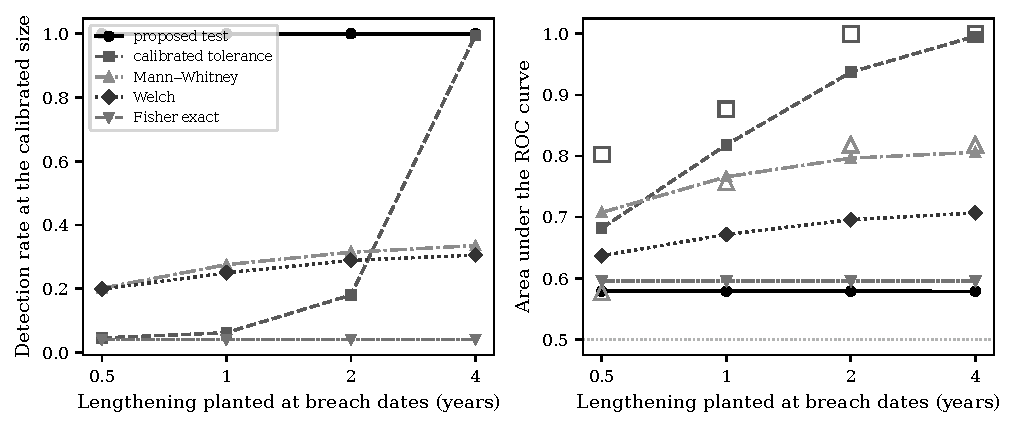
\includegraphics[width=0.95\textwidth]{fitted-power}
\caption{Detection rate at the calibrated size (left) and area under the ROC curve (right) against the size of a lengthening planted at breach dates, for the proposed test, the calibrated tolerance and three published tests on the simulated banks (lines), with the areas on the real fitted series for the tolerance and the Mann--Whitney test as open markers.}
\label{fig:fitted-power}
\end{figure}

Figure~\ref{fig:fitted-power} shows the same results as curves: the proposed test is flat at an area of \fitAucCEngine{} whatever the size of the lengthening, the published tests reach areas between \fitAucDFisher{} and \fitAucDMw{} at 4 years, and the tolerance rule passes them between 0.5 and 1 year and reaches \fitAucDTol{} at 4 years.

The tolerance rule restores the discrimination for overrides larger than the natural changes. Calibrated at 5\,\% on 1,000 separate banks at the breach prevalence of 0.25, its tolerance is \deltaB{} years and it flags \fitNullTol{} of the null banks (\fitNullLoTol{} to \fitNullHiTol{}\,\%), so the size holds (prediction H7). It flags \fitAddATol{}, \fitAddBTol{}, \fitAddCTol{} and \fitAddDTol{} of the banks with a lengthening of 0.5, 1, 2 and 4 years, and its areas are \fitAucATol{}, \fitAucBTol{}, \fitAucCTol{} and \fitAucDTol{}: at 1 year it flags only \fitAddBTol{}, at 2 years \fitAddCTol{} of the overrides, and at 4 years nearly all. The look-ahead variant is within one percentage point of it at every size. On the real fitted series, whose changes never exceed \realMaxChange{} years, the tolerance calibrated on the simulated banks is too large: it flags \realTolNull{} of the null draws, \realTolAddB{} of those with a 1-year lengthening, \realTolAddC{} of those with 2 years and \realTolAddD{} of those with 4 years, while its area is \realTolAucB{} at 1 year and \realTolAucC{} at 2 years. The threshold-free ranking is therefore excellent on the real series and the calibrated threshold is conservative, because the simulated population has larger changes than the real bank; the size is held and the power is lost. On the same draws the proposed test flags \realEngineNull{} of the null draws and has an area of \realEngineAuc{}, and the Mann--Whitney test flags \realMwNull{} of them with an area of \realMwAucC{} at 2 years.

The override that moves the weights toward the longest tranche (Table~\ref{tab:weight-override}) is the case that none of the detectors reads. In \invisShare{} of the histories the planted date finds the fitted weights already on the longest tranche, so that nothing changes; elsewhere the override lengthens the maturity by a fraction of the distance to the cap and shrinks every later change. The proposed test has an area of \wEngineAucLow{} at the smallest share and \wEngineAucHigh{} at the largest, below one half because the override creates ties; the stability test flags \wStabFlagHigh{} of the banks at the largest share with an area of \wStabAucHigh{}; the tolerance rule flags \wTolFlagHigh{} with an area of \wTolAucHigh{}, and the Mann--Whitney test has an area of \wMwAucHigh{}. This override is not detected by any method here, and it is the form that an override toward the cap of a standardised grid takes.

\begin{table*}[htbp]
\centering
\footnotesize
\caption{An override that moves the replicating-portfolio weights toward the longest tranche at breach dates (breach prevalence 0.25, 2,000 banks): the share of histories in which the override leaves the weights unchanged because they already sit on that tranche, and the flag rate and area under the ROC curve of the detectors that can read it.}
\label{tab:weight-override}
\resizebox{\textwidth}{!}{%
\begin{tabular}{rrrrrrrrr}
\toprule
Share $s$ & Invisible (\%) & Engine flags (\%) & Engine AUC & Stability flags (\%) & Stability AUC & Tolerance flags (\%) & Tolerance AUC & Mann--Whitney AUC \\
\midrule
0.05 & 22.1 & 83.4 & 0.506 & 47.6 & 0.483 & 3.2 & 0.498 & 0.519 \\
0.1 & 22.1 & 83.4 & 0.506 & 45.4 & 0.467 & 2.5 & 0.502 & 0.537 \\
0.2 & 22.1 & 83.0 & 0.498 & 40.6 & 0.442 & 2.4 & 0.521 & 0.576 \\
0.4 & 22.1 & 81.5 & 0.457 & 43.2 & 0.437 & 2.5 & 0.564 & 0.604 \\
\bottomrule
\end{tabular}}
\end{table*}


Table~\ref{tab:robustness} reports what happens when the breach prevalence of the bank is not that of the calibration. At the calibration prevalence of 0.25 the tolerance flags \fitNullBTol{} of the null banks; calibrated at the prevalence tested it flags \fitNullATol{} at 0.10 and \fitNullCTol{} at 0.50; calibrated at 0.25 and applied to the other prevalences it flags \fitMisATol{} and \fitMisCTol{} (upper end \fitMisCTolHi{} at 0.50), so the size is exceeded at the high prevalence and prediction H8, a rate of at most 5\,\% at every prevalence, is refuted by the point estimate while the interval includes 5\,\%. A tolerance rule is calibrated for a breach process and not for a bank. For the override one date before the planted breach, the tolerance flags \earlyTol{} of \earlyN{} banks and its look-ahead variant \earlyTolLa{}, a ratio of \earlyRatio{}, so prediction H9, a ratio of at least 1.5, is refuted; the proposed test and the breach-agnostic count flag \earlyEngine{} and \ablEarlyAny{}, which tells nothing about the override because they flag nearly all null banks.

\begin{table*}[htbp]
\centering
\footnotesize
\caption{False-flag rates on 2,000 held-out simulated banks at three breach prevalences: the tolerance rule calibrated on 1,000 banks at the prevalence tested and at 0.25 with 95\% Wilson intervals, and the published tests at their nominal 5\% size together with the red limit of the weight stability test.}
\label{tab:robustness}
\resizebox{\textwidth}{!}{%
\begin{tabular}{rrrccrrrr}
\toprule
\multicolumn{3}{l}{} & \multicolumn{2}{c}{Tolerance false flags (\%)} & \multicolumn{4}{c}{Other detectors, false flags (\%)} \\
\cmidrule(lr){4-5}\cmidrule(lr){6-9}
Prevalence & Mean $m$ & $\delta$ (years) & Calibrated here & Calibrated at 0.25 & Fisher & Mann--Whitney & Welch & Weight stability \\
\midrule
0.1 & 3.92 & 2.17 & 4.7 (3.9, 5.7) & 3.4 (2.7, 4.3) & 1.8 & 8.2 & 6.5 & 49.8 \\
0.25 & 4.41 & 2.47 & 3.9 (3.1, 4.8) & 3.9 (3.1, 4.8) & 2.1 & 7.2 & 6.0 & 49.8 \\
0.5 & 5.80 & 2.61 & 4.7 (3.9, 5.7) & 5.5 (4.6, 6.6) & 1.5 & 6.6 & 5.9 & 49.8 \\
\bottomrule
\end{tabular}}
\end{table*}


\subsection{Checks of the propositions}
\label{sec:res-theory}

Table~\ref{tab:theory-checks} compares the closed forms with simulation. The probability of Equation~\eqref{eq:hypergeometric} (Figure~\ref{fig:hypergeometric}) lies inside the interval of the simulated placement rate in \hyperInside{} of \hyperCells{} pairs $(k,m)$, and the one outside lies \hyperOutGap{} percentage points from its interval, as expected of \hyperCells{} 95\,\% intervals, which miss about one comparison in twenty. The detection probability of Equation~\eqref{eq:gaussian-power} differs from simulation by at most \gaussWorst{} over the \gaussPoints{} points of Figure~\ref{fig:gaussian-power}. The one-sided Fisher p-value equals the permutation p-value to within \fisherPermMax{} on \fisherPermN{} random histories (Proposition~\ref{prop:association}). The mean false-flag rate of the calibrated tolerance over \confCalibrations{} calibrations of \confNcal{} histories is \confMean{}, against \confTheory{} from Equation~\eqref{eq:conformal}; the realised rate of one calibration ranges from \confLo{} to \confHi{} (2.5th to 97.5th percentile), with a largest value of \confMax{}, and \confShareAbove{} of the calibrations exceed 5\,\%, as the bound on the average allows (Figure~\ref{fig:conformal-validity}).

\begin{table}[htbp]
\centering
\footnotesize
\caption{The closed forms of Propositions~\ref{prop:false-flag}, \ref{prop:gaussian} and \ref{prop:conformal} against simulation: the probability that a change falls on a breach date under uniform placement (100,000 placements), the power of the tolerance rule on Gaussian changes (200,000 histories) and the mean false-flag rate of the calibrated tolerance over 500 calibrations of 1,000 maxima of three Gaussian changes, with the 2.5 and 97.5 percentiles of the realised rate.}
\label{tab:theory-checks}
\begin{tabular}{lcc}
\toprule
Quantity & Closed form & Simulation (95\% interval) \\
\midrule
\relax Placement: $n=11$, $k=1$, $m=1$ & 0.0909 & 0.0925 (0.0907, 0.0943) \\
\relax Placement: $n=11$, $k=1$, $m=4$ & 0.3636 & 0.3644 (0.3614, 0.3674) \\
\relax Placement: $n=11$, $k=2$, $m=2$ & 0.3455 & 0.3460 (0.3430, 0.3489) \\
\relax Placement: $n=11$, $k=3$, $m=4$ & 0.7879 & 0.7873 (0.7847, 0.7898) \\
\relax Placement: $n=11$, $k=5$, $m=6$ & 0.9978 & 0.9975 (0.9971, 0.9978) \\
\relax Gaussian power: $m=1$, $\mu/\sigma=1$ & 0.1701 & 0.1693 \\
\relax Gaussian power: $m=1$, $\mu/\sigma=2$ & 0.5160 & 0.5151 \\
\relax Gaussian power: $m=1$, $\mu/\sigma=4$ & 0.9793 & 0.9794 \\
\relax Gaussian power: $m=3$, $\mu/\sigma=1$ & 0.1138 & 0.1138 \\
\relax Gaussian power: $m=3$, $\mu/\sigma=2$ & 0.3710 & 0.3690 \\
\relax Gaussian power: $m=3$, $\mu/\sigma=4$ & 0.9483 & 0.9477 \\
\relax Gaussian power: $m=6$, $\mu/\sigma=1$ & 0.0913 & 0.0919 \\
\relax Gaussian power: $m=6$, $\mu/\sigma=2$ & 0.2948 & 0.2969 \\
\relax Gaussian power: $m=6$, $\mu/\sigma=4$ & 0.9181 & 0.9189 \\
Calibrated tolerance: mean false-flag rate, 500 calibrations & 0.0500 & 0.0506 (0.0373, 0.0650) \\
\bottomrule
\end{tabular}
\end{table}


\begin{figure}[htbp]
\centering
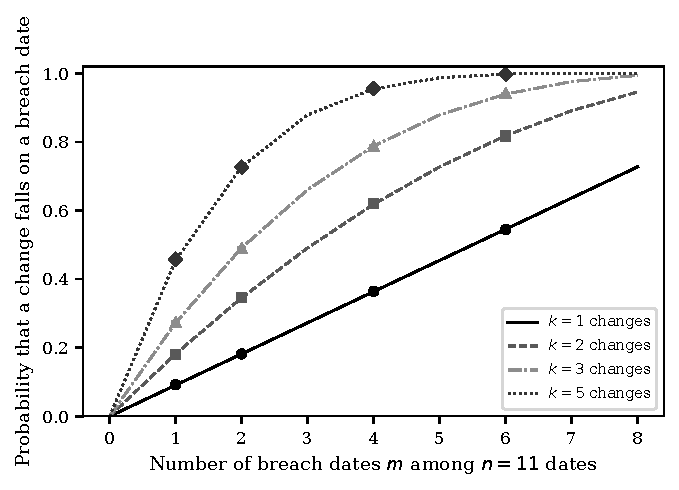
\includegraphics[width=0.62\textwidth]{hypergeometric}
\caption{The probability that at least one change falls on a breach date, from Equation~\eqref{eq:hypergeometric}, against the number of breach dates among 11 dates, for one, two, three and five changes (lines), with the simulated placements as markers and their 95\% Wilson intervals.}
\label{fig:hypergeometric}
\end{figure}

\begin{figure}[htbp]
\centering
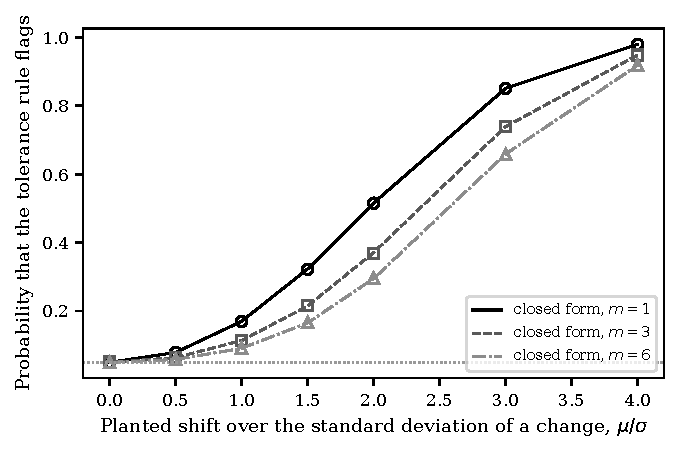
\includegraphics[width=0.62\textwidth]{gaussian-power}
\caption{The probability that the tolerance rule flags Gaussian changes against the planted shift in units of their standard deviation, for one, three and six breach dates, with the closed form of Equation~\eqref{eq:gaussian-power} as lines and the simulation as open markers; the dotted line is the size of 5\%.}
\label{fig:gaussian-power}
\end{figure}

\begin{figure}[htbp]
\centering
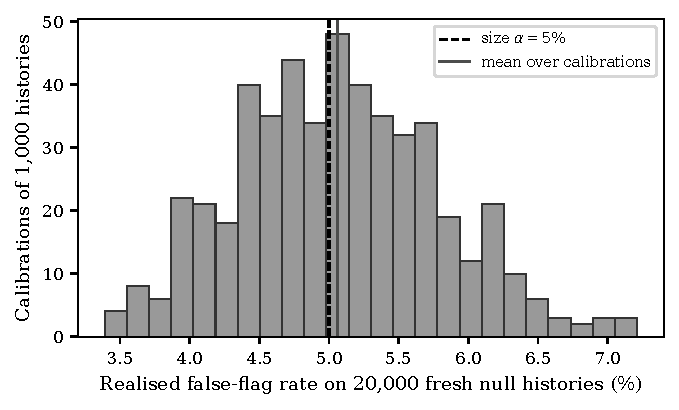
\includegraphics[width=0.62\textwidth]{conformal-validity}
\caption{The realised false-flag rate on \confNtest{} fresh null histories of each of \confCalibrations{} independent calibrations of the tolerance on \confNcal{} null histories each, with the size of 5\% and the mean over the calibrations marked.}
\label{fig:conformal-validity}
\end{figure}

\subsection{Outcome of the predictions}
\label{sec:res-hypotheses}

Table~\ref{tab:hypotheses} gives the nine predictions with their measured values: \hypothesesHeld{} held and \hypothesesRefuted{} were refuted. H1 to H4 and H7 held. H5, H6, H8 and H9 were refuted, and each refutation is a result about the limits of the test: its false-flag rate on a stated parameter is not at the conventional size, it does not discriminate on a re-estimated parameter, a calibrated tolerance does not transfer across breach prevalences without a loss of size, and reading one date ahead does not recover an anticipated override. The five that held are the specification of the test and the closed forms that follow from it: the reproduction of the committed rows and of the definition on every history enumerated, the detection of one on a stated parameter, the closed form of the false-flag rate, and the size of the calibrated tolerance together with its detection of large overrides. The four that failed are the predictions that a validator would make by treating the test as a statistical test of a re-estimated parameter, and each failure traces to a proposition: H5 to Proposition~\ref{prop:false-flag}(c), H6 to Proposition~\ref{prop:degeneracy}, H8 to the exchangeability that Proposition~\ref{prop:conformal} requires, and H9 to the single change that a persistent override produces. The outcomes are decided by code from the committed results, with the criteria of Table~\ref{tab:hypotheses}, so that a rerun that changed a rate across a criterion would change the outcome in the table.

\begin{table}[htbp]
\centering
\footnotesize
\caption{The nine predictions tested, with the criterion that decides each, the value measured by the experiments of this work and the outcome; the experiments are on the stored history of case C14, on constructed and enumerated histories and on 4,000 simulated histories per cell. A dagger marks a prediction formulated after a first run of the re-estimated experiment had been inspected (Section~\ref{sec:design-hypotheses}).}
\label{tab:hypotheses}
\begin{tabular}{@{}l p{4.6cm} p{3.2cm} p{3.1cm} l@{}}
\toprule
ID & Prediction & Criterion & Measured & Outcome \\
\midrule
H1 & The test is not evaluated at 2021-Q4, red at 2022-Q2 with one change and red at 2022-Q4 with two; the held core share and core maturity are not flagged & all three stored rows and the two held parameters reproduced by the engine on the stored series & 3 of 3 rows; 2 of 2 held parameters & held \\
H2 & Green for a parameter held through a breach, for a change with no breach and for a change before the breach; red for a change at the breach; the stored series with its breach flags set to false is green & all constructed histories, every history of a binary grid, 20,000 random histories and the control agree with the closed-form count & 8 of 8 histories; 0 disagreements in 22,728 & held \\
H3 & On a stated parameter the test flags every history in which an assumption was changed at a breach date & lower end of the 95\% interval of the detection at least 99\% in every cell & lowest lower bound 99.9\% over 11 cells & held \\
H4 & The false-flag rate on a stated parameter with changes unrelated to breaches equals $E[1-(1-\lambda)^m]$ (Proposition~\ref{prop:false-flag}) & the closed form inside the 95\% interval of the measured rate in at least 10 of 11 cells (an interval misses one cell in twenty), a cell outside re-run under three further seeds & 10 of 11 cells; the one outside inside the interval under 3 of 3 further seeds & held \\
H5 & The false-flag rate of the test on a stated parameter with unrelated changes is at most 5\% & the point estimate at most 5\% in every cell & 17.0 to 66.3\% & refuted \\
H6$^\dagger$ & On a re-estimated parameter the test separates a 2-year override at breach dates from none & area under the ROC curve at least 0.70 & 0.579 (0.561, 0.595) & refuted \\
H7$^\dagger$ & The tolerance rule calibrated at 5\% holds its size on held-out banks and flags a 4-year override & false-flag rate at most 5\% and detection of at least 90\% & 3.9\% false flags; 99.5\% detection & held \\
H8$^\dagger$ & The tolerance calibrated at breach prevalence 0.25 keeps its size at prevalences 0.10 and 0.50 & point estimate of the false-flag rate at most 5\% at every prevalence & 3.4 to 5.5\% (at 0.50, 95\% interval 4.6 to 6.6\%) & refuted \\
H9$^\dagger$ & A one-date look-ahead recovers a 4-year override made at the date before a breach begins & detection at least 1.5 times that of the same-date rule & 91.0\% against 3.7\% (ratio 24.9) & held \\
\bottomrule
\end{tabular}
\end{table}

